% Figure 1 (text width). File: figures/fig_main_tokens.pdf from the figures agent (stand-in: f1_vs_tokens.pdf until delivered).
\begin{figure*}[t]
  \centering
  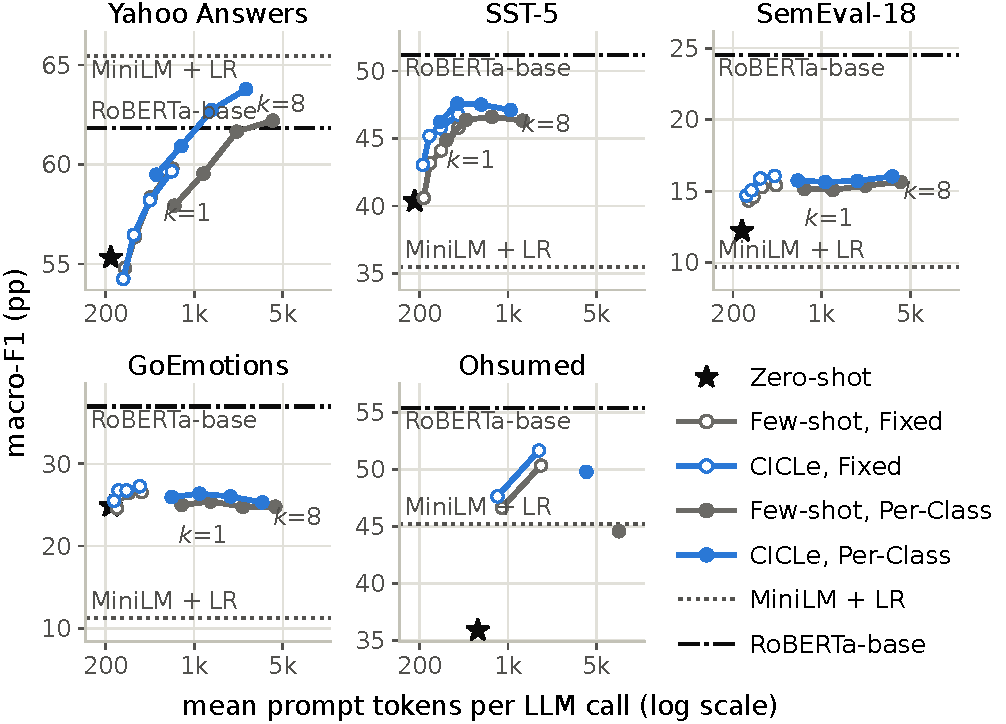
\includegraphics[width=0.8\textwidth]{figures/fig_main_tokens.pdf}
  \caption{Macro-F1 against mean prompt tokens per LLM call (log scale), one panel per dataset. Each point is one method, retrieval variant and $k$ at the reference setting, averaged over six models and three seeds, with $k$ increasing along each line. Grey is few-shot prompting, blue CICLe, hollow markers Fixed and filled markers Per-Class retrieval. Horizontal lines are the base classifier and fine-tuned RoBERTa-base. Ohsumed Per-Class is $k = 1$ only. Bootstrap intervals are in Table~\ref{tab:main}.}
  \label{fig:main_tokens}
\end{figure*}
